\documentclass{article}
\usepackage[utf8]{inputenc}
\usepackage{amsmath,hyperref,verbatim,listings,graphicx,subfigure,fullpage}

\begin{document}

\title{UML computer project 1}
\author{
Juha-Antti Isojärvi\\
???
\and
Mikko Sysikaski\\
013573016\\
Department of Computer Science\\
Master student}
\date{}
\maketitle

\section{Exercise 1}
\subsection{}
The plots are shown in Figure~\ref{fig:scatter}. The covariance matrices where generated with the Stetson-Harrison method.
\subsection{}
The principal components of the first and the third point set are shown in Figure~\ref{fig:pcadir}.
\subsection{}
The Figure~\ref{fig:histo} contains the histograms obtained by projecting the points of the first point set on its principal components.
\subsection{}
\subsection{}

\newcommand{\sscale}{0.5}
\begin{figure}\centering
	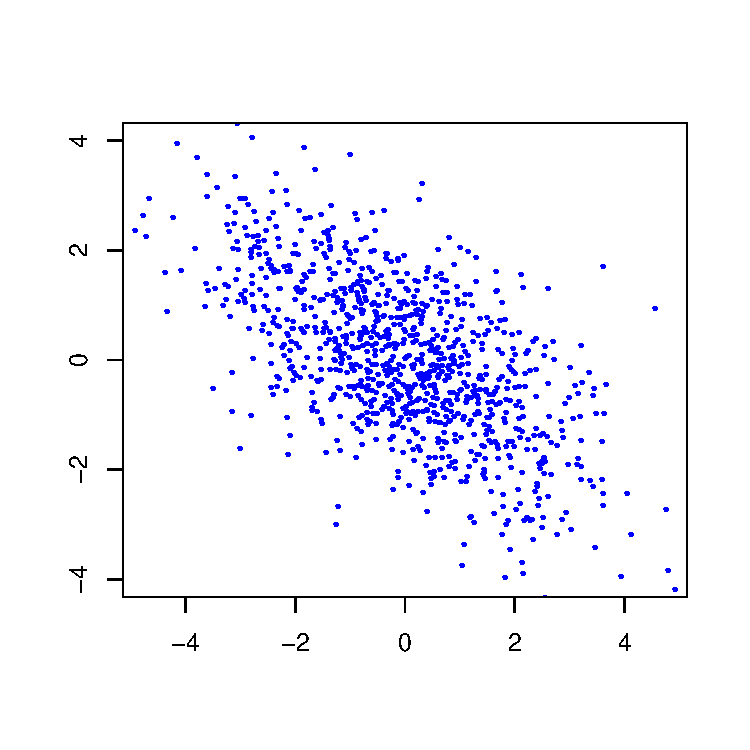
\includegraphics[scale=\sscale]{scatter1}
	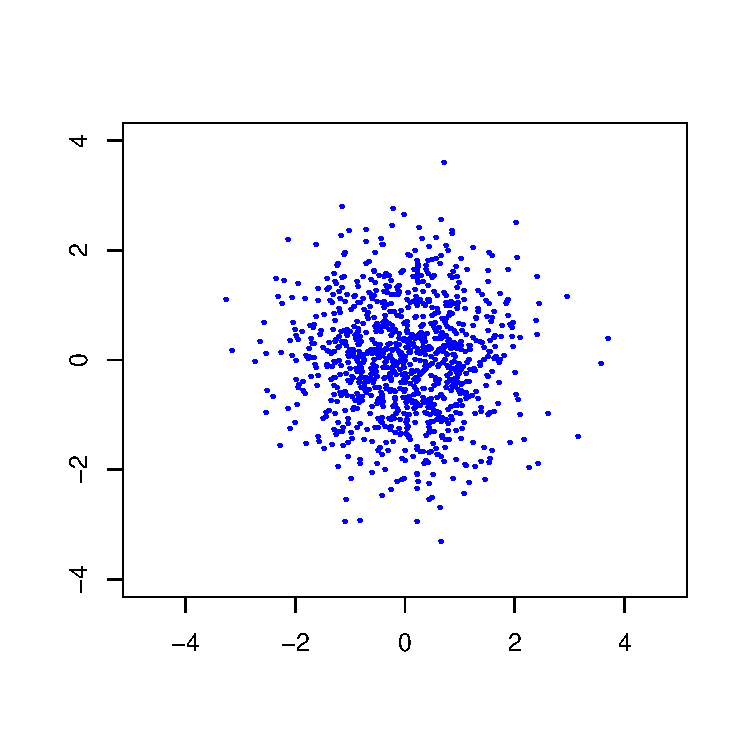
\includegraphics[scale=\sscale]{scatter2}

	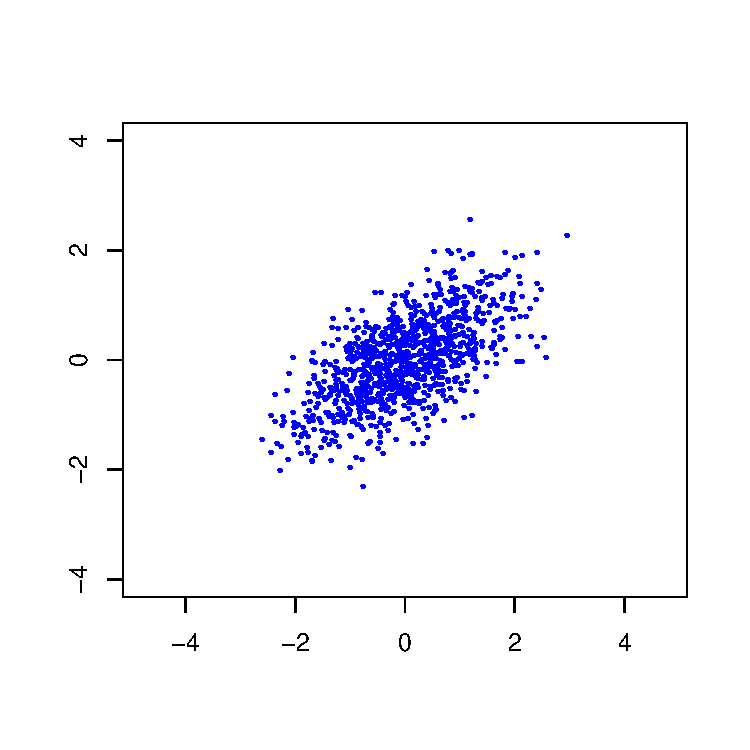
\includegraphics[scale=\sscale]{scatter3}
	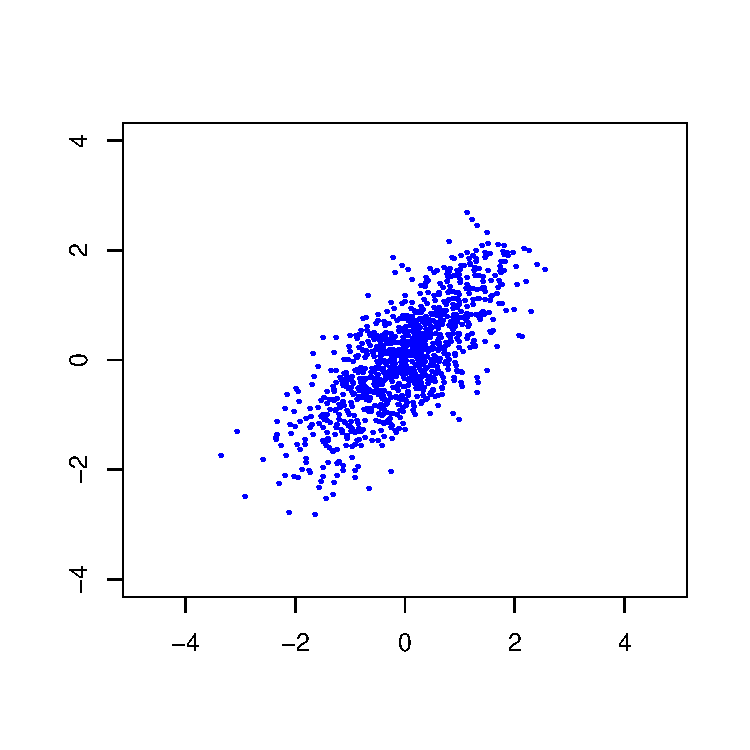
\includegraphics[scale=\sscale]{scatter4}
	\caption{The scatter plots of the data generated in task 1.1.} \label{fig:scatter}
\end{figure}
\begin{figure} \centering
	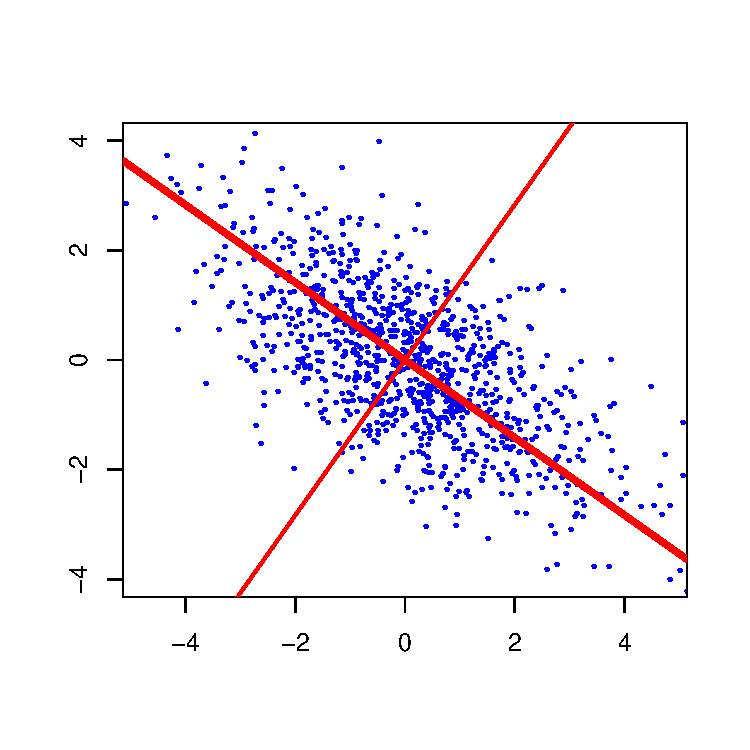
\includegraphics[scale=\sscale]{pcadir1}
	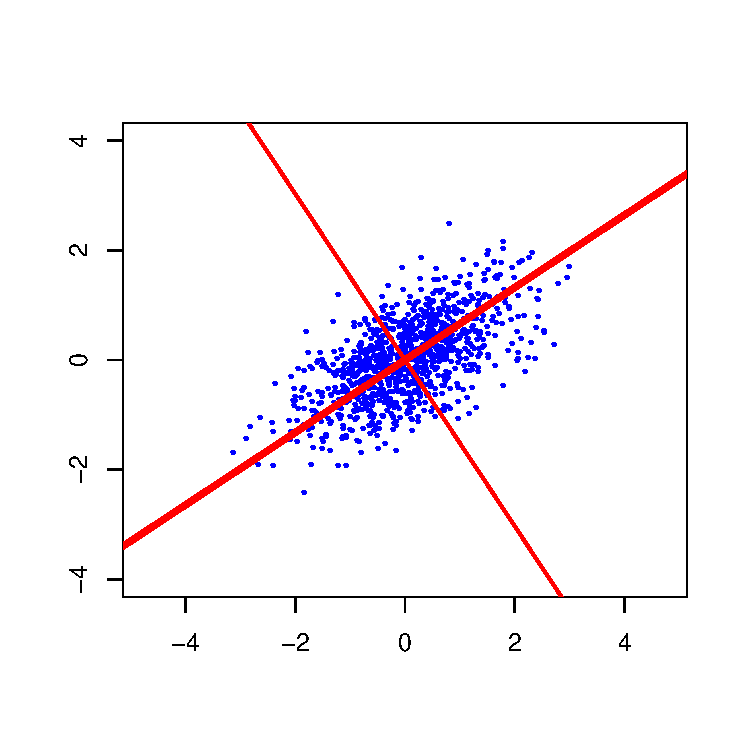
\includegraphics[scale=\sscale]{pcadir3}
	\caption{Principal components of the first and the third point set. The first PC is the bolder line.} \label{fig:pcadir}
\end{figure}
\begin{figure} \centering
	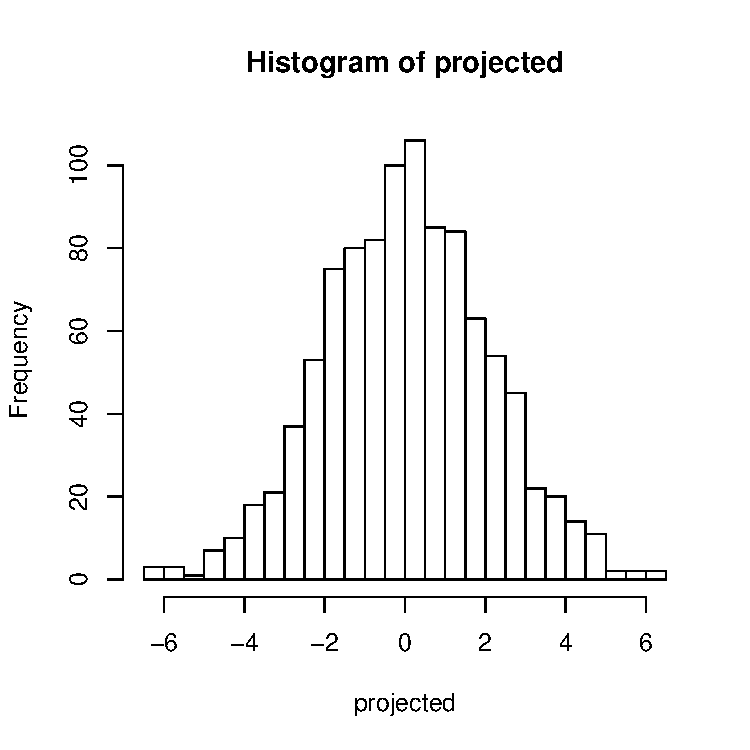
\includegraphics[scale=\sscale]{histo1-1}
	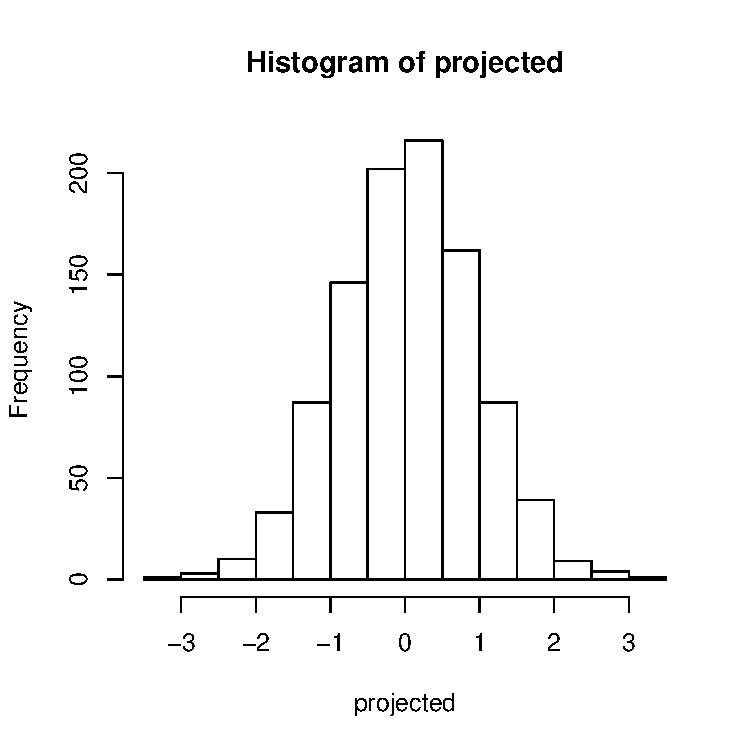
\includegraphics[scale=\sscale]{histo1-2}
	\caption{Histograms of the 1-dimensional data obtained by projecting the points of the first point set on its principal components.} \label{fig:histo}
\end{figure}
\begin{figure} \centering
	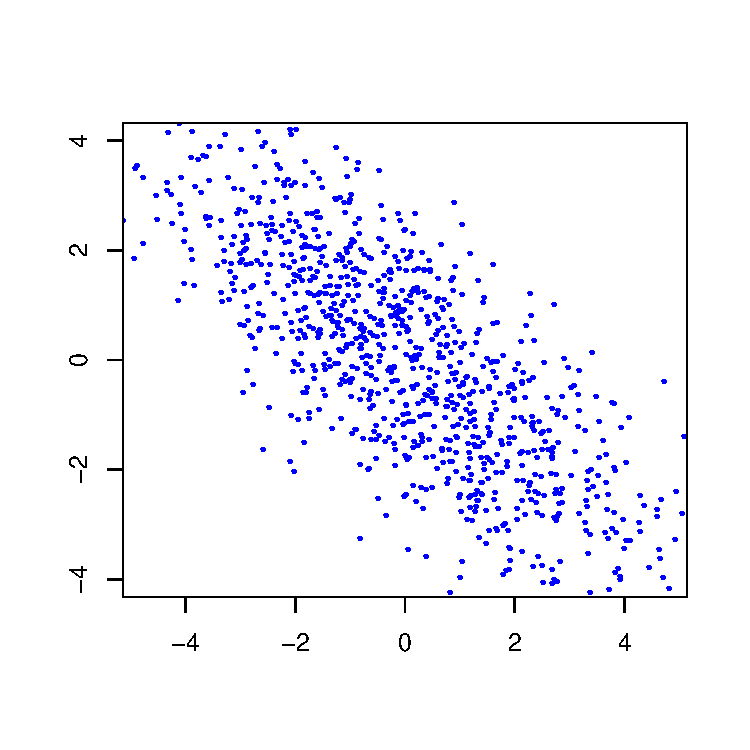
\includegraphics[scale=\sscale]{vscatter}
	\caption{} \label{fig:vscatter}
\end{figure}
\begin{figure} \centering
	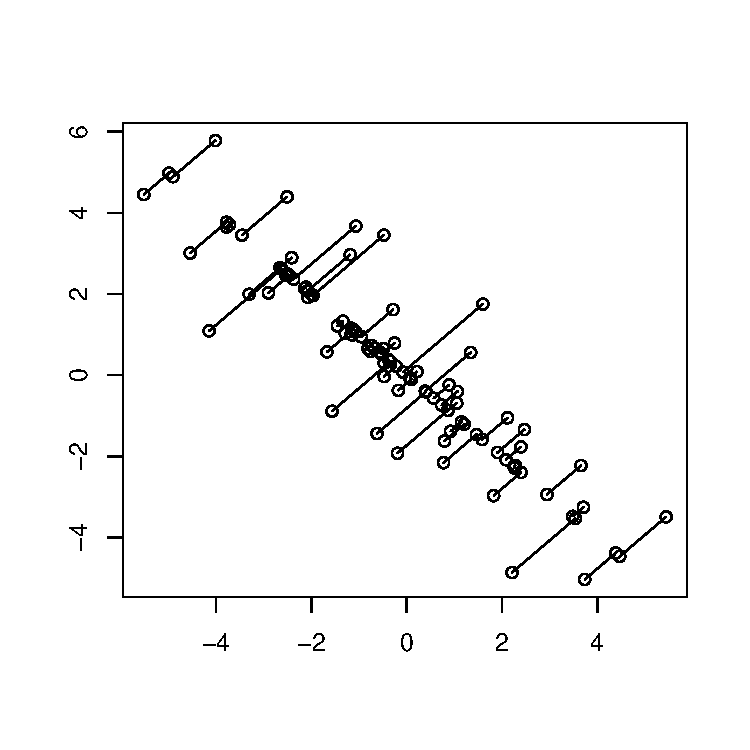
\includegraphics[scale=\sscale]{proj}
	\caption{} \label{fig:proj}
\end{figure}

\section{Exercise 2}
\newcommand{\X}{\ensuremath{\mathbf{X}}}
\subsection{}
The task was to do primary component analysis on the matrix
$$ X =
\begin{pmatrix}
	5 & 3 & 0 & 1 & -1 & -3 & 5 & 0 & -4 & -4 \\
	-2 & -1 & 0 & 0 & 1 & 4 & -3 & 1 & 5 & 3 \\
	0 & 1 & 4 & -1 & 0 & 5 & 5 & -5 & -3 & -3 \\
	0 & 2 & 3 & 0 & -1 & 3 & 3 & -7 & -2 & 0 \\
	3 & 4 & -2 & 1 & 3 & -3 & -3 & 2 & 0 & 0
\end{pmatrix}.
$$

The Figure~\ref{fig:42} displays the data and the original variables projected to the first two principal components.
\subsection{}
The amount of variance explained as a function of the number of principal components used is displayed in Figure~\ref{fig:varamount}. It can be seen that the projection to the first two components in Figure~\ref{fig:42} convey about 90.6\% of the information of the data.
\subsection{}
\subsection{}
The quartimax applied to the first two principal components of \X. Figure~\ref{fig:qmax} shows the projections of the variables on the rotated components. Note that the figure is the same as Figure~\ref{fig:42}, only rotated. The rotation doesn't change the subspace spanned by the principal components, so they explain the same amount of variance before and after rotation.

\begin{figure}\centering
	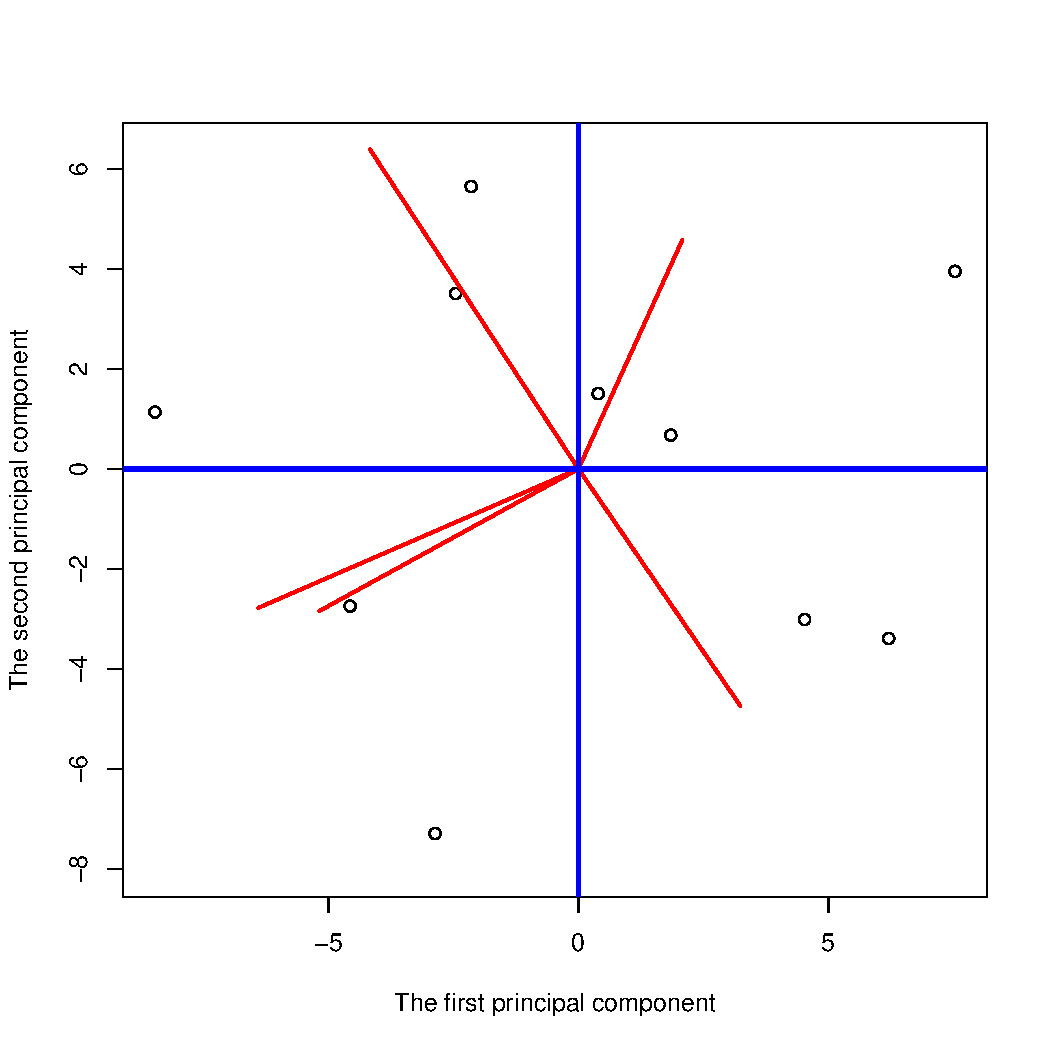
\includegraphics[scale=\sscale]{fig42}
	\caption{Reproduction of Figure~4.2 on the lecture notes. The blue points are the data points projected to the first two principal components. The red lines are the projections of the original coordinate axes.}\label{fig:42}
\end{figure}
\begin{figure}\centering
	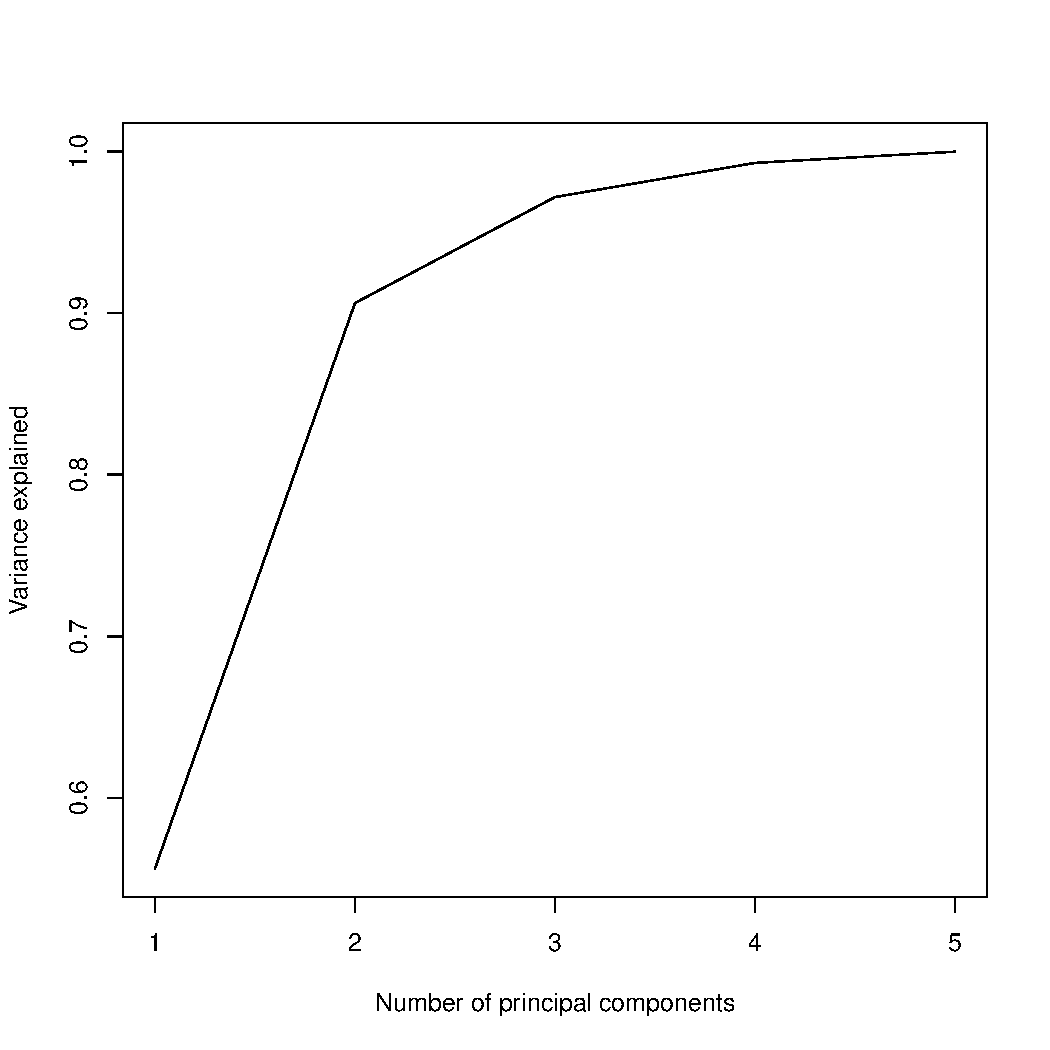
\includegraphics[scale=\sscale]{varamount}
	\caption{The proprotion of the variance explained by using only some of the principal components.}\label{fig:varamount}
\end{figure}
\begin{figure}\centering
	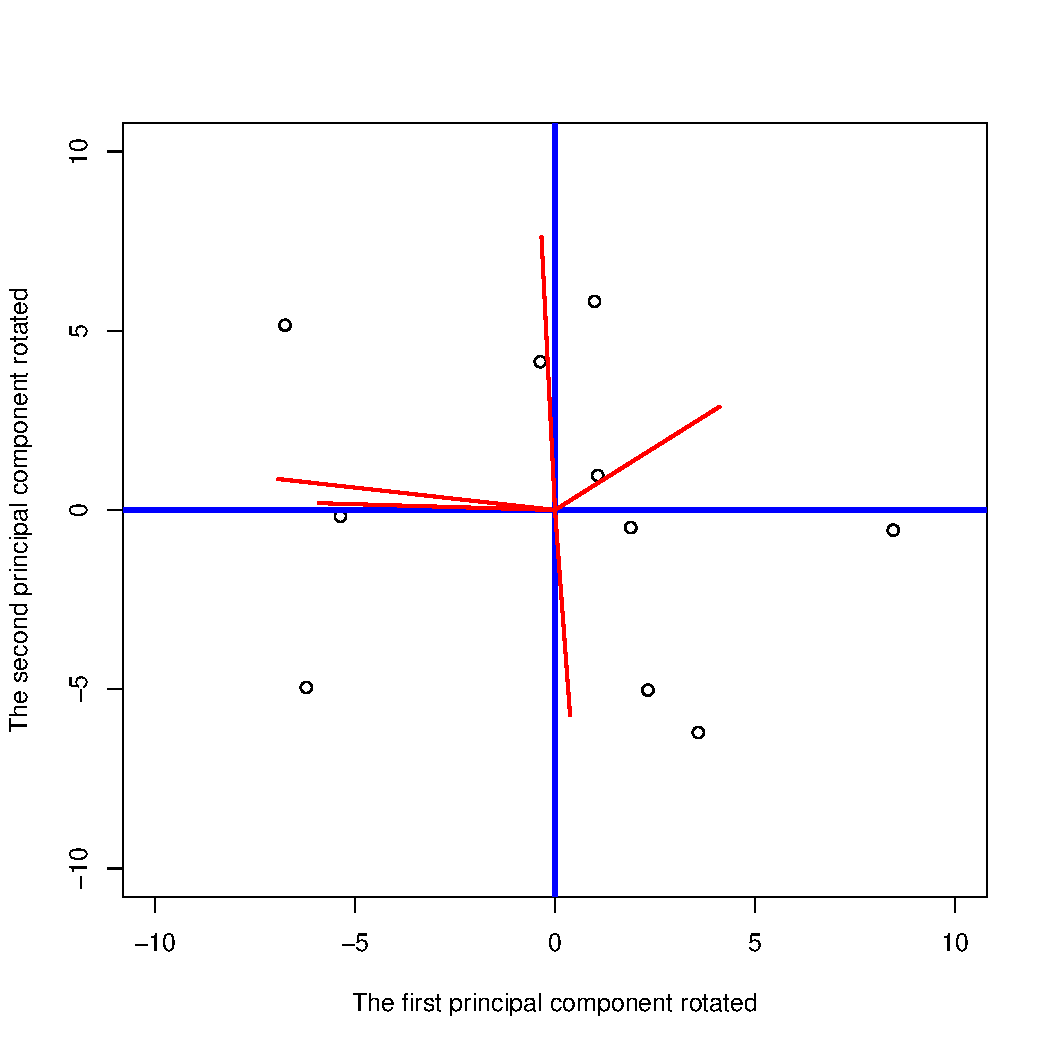
\includegraphics[scale=\sscale]{qmax}
	\caption{The projection to principal components after rotating them using the quartimax algorithm to have the original variables as close to the new coordinate axes as possible.}\label{fig:qmax}
\end{figure}

\section{Exercise 3}
\subsection{}
\subsection{}
\subsection{}
\subsection{}

\begin{figure}\centering
	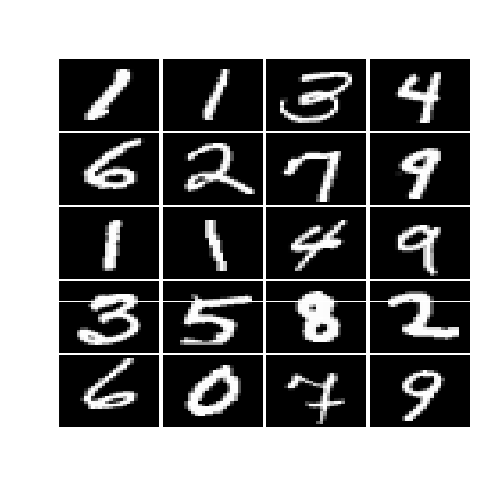
\includegraphics[scale=0.4]{digits}
	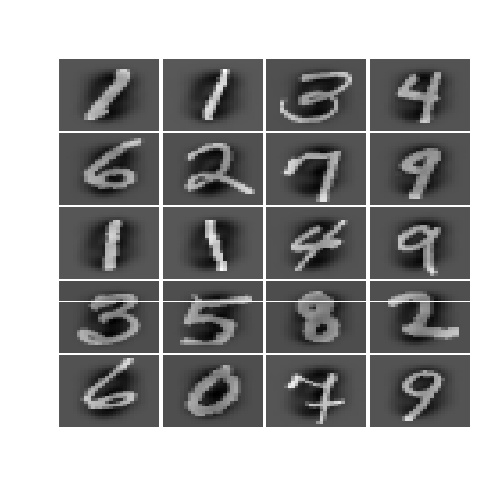
\includegraphics[scale=0.4]{digitspre}
	\caption{}\label{fig:digits}
\end{figure}
\begin{figure}\centering
	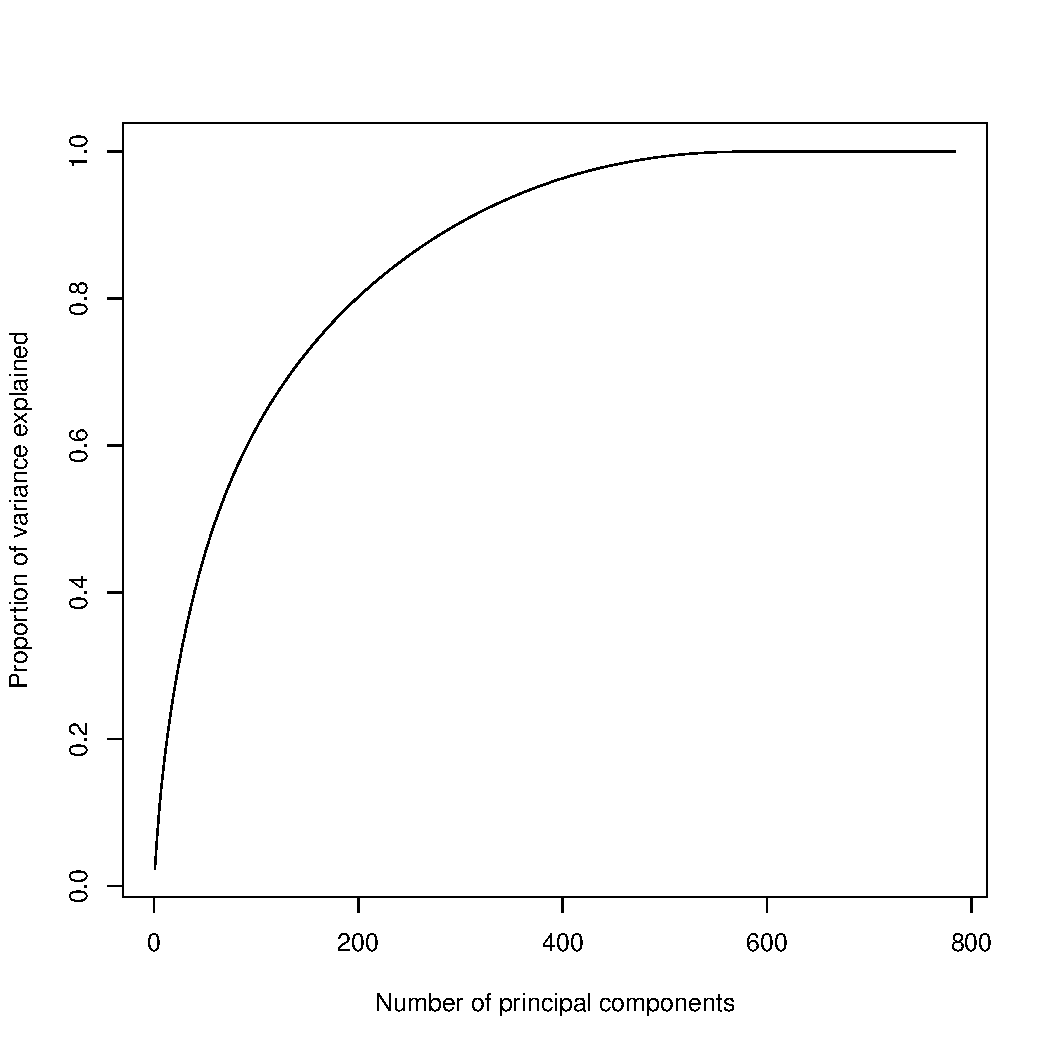
\includegraphics[scale=0.4]{pcavar}
	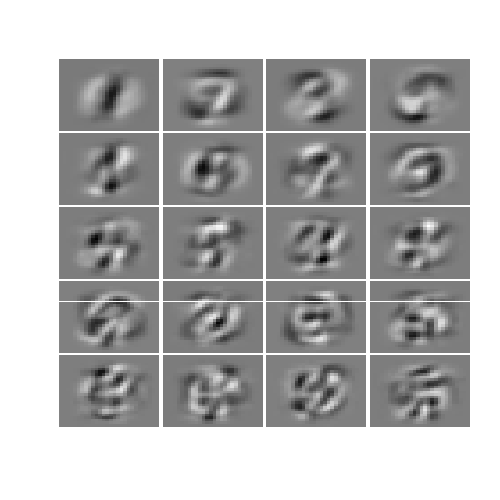
\includegraphics[scale=0.4]{pcanums}
	\caption{}\label{fig:pcavar}
\end{figure}
\begin{figure}\centering
	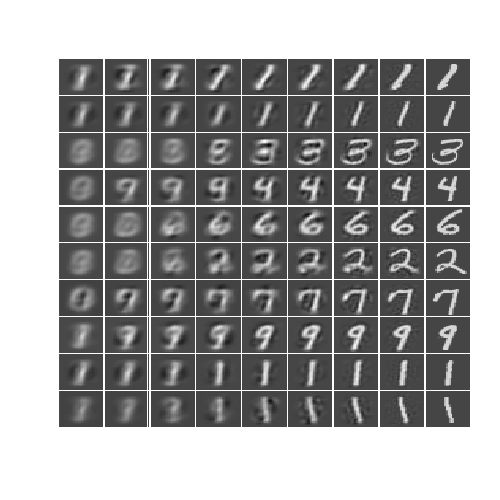
\includegraphics[scale=\sscale]{digitreduce}
	\caption{}\label{fig:reduce}
\end{figure}
\begin{figure}\centering
\newcommand{\dns}{0.4}
	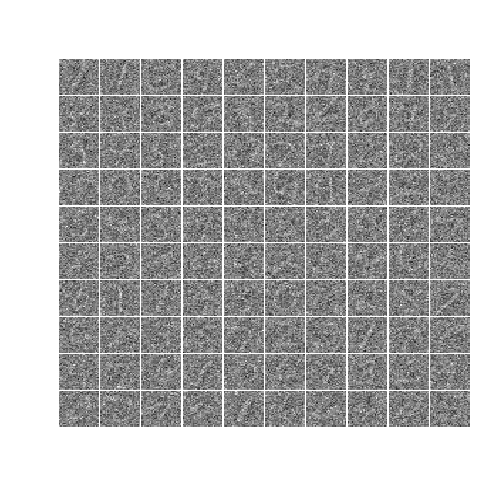
\includegraphics[scale=\dns]{noisy}
	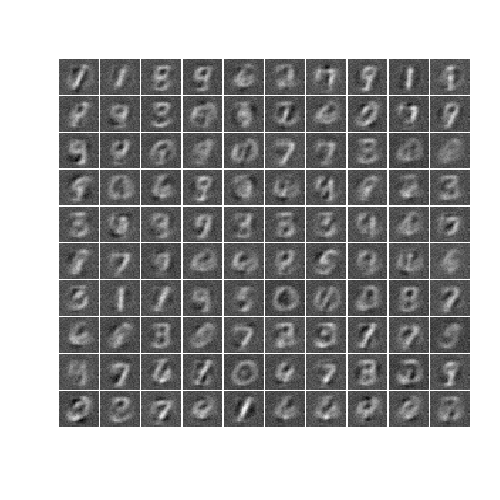
\includegraphics[scale=\dns]{denoise8}
	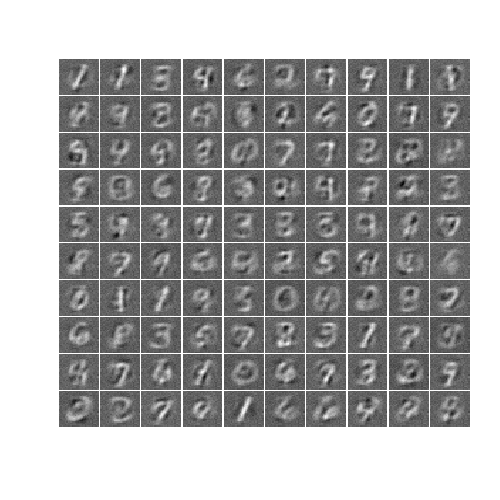
\includegraphics[scale=\dns]{denoise16}
	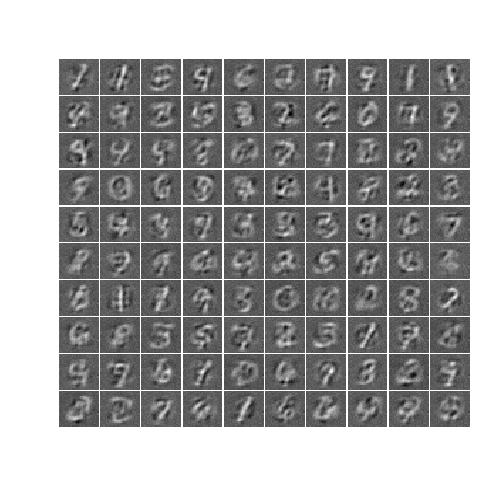
\includegraphics[scale=\dns]{denoise32}
%	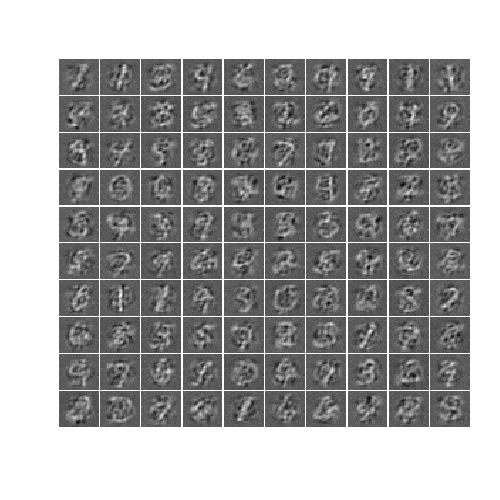
\includegraphics[scale=\dns]{denoise64}
	\caption{}\label{fig:denoise}
\end{figure}

\end{document}
